Mira el siguiente gráfico.

\begin{figure}[h!]
    \centering
	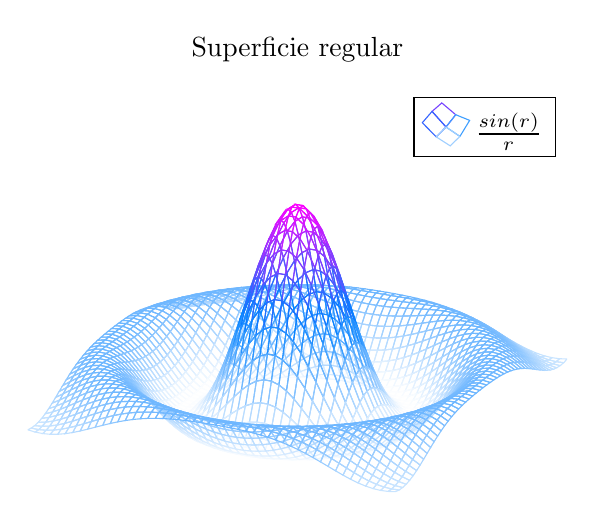
\begin{tikzpicture}
	\begin{axis}[
	    title=Superficie regular,
	    hide axis,
	    colormap/cool,
	]
	\addplot3[
	    mesh,
	    samples=50,
	    domain=-8:8,
	]
	{sin(deg(sqrt(x^2+y^2)))/sqrt(x^2+y^2)};
	\addlegendentry{\(\frac{sin(r)}{r}\)}
	\end{axis}
	\end{tikzpicture}
    \caption{Gráfico de superficie usando tikz}
    \label{fig:scientif}
\end{figure}